% VARIABLES %%%
\def\theme{\large Brevet Amerique du Nord 31 mai 2023 (Exercice 4)}
\def\date{17/05/2024}
\def\authors{\fsize{8pt}
    CADOT - COURTIN - PESIN
}

% Define the petal shape
\newcommand{\petal}{%
    \draw(0,0) -- (0.9,0) -- (1.1,0.4) -- (0.2,0.4) -- cycle;
}

%%%%%%%%%%%%%%%

% \textbf{Exercice 4 \hfill 20 points}

\medskip

À l'aide d'un logiciel de programmation, on veut réaliser le motif \og Fleur\fg suivant.

\begin{center}
    \begin{tabular}{|c|}\hline
        \textbf{Motif \og Fleur \fg}\\
        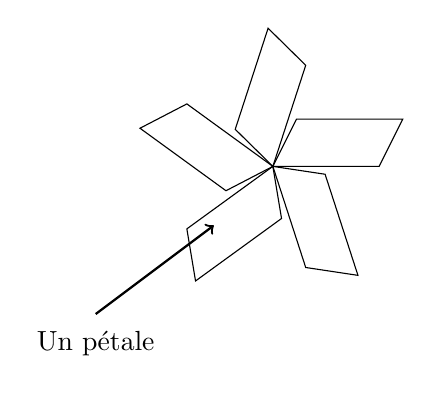
\begin{tikzpicture}[scale = 1.5]
            % Draw five petals rotated around the origin
            \foreach \angle in {0,72,...,288} {
            \begin{scope}[rotate=\angle]
                \petal
            \end{scope}
            }
        
            % Add the label and arrow
            \node at (-1.5,-1.5) {Un pétale};
            \draw[thick,->] (-1.5,-1.25) -- (-0.5,-0.5);
        \end{tikzpicture}\\ \hline
    \end{tabular}
\end{center}

\begin{enumerate}
\item 
	\begin{enumerate}
		\item Le parallélogramme KLMN ci-dessous représente un des pétales du motif \og Fleur \fg.
        Construire ce parallélogramme sur la copie en prenant $1$~cm pour 5 pas.
        \begin{center}
            \begin{tikzpicture}[scale = 1]
                % Define the coordinates for the parallelogram
                \coordinate (K) at (0,0);
                \coordinate (L) at (7,0);
                \coordinate (M) at (9,3.5);
                \coordinate (N) at (2,3.5);
              
                % Draw the parallelogram
                \draw (K) -- (L) -- (M) -- (N) -- cycle;
              
                % Label the points
                \node at (K) [below left] {K};
                \node at (L) [below right] {L};
                \node at (M) [above right] {M};
                \node at (N) [above left] {N};
              
                % Add text for distances
                \node at ($(K)!0.5!(L)$) [below] {35 pas};
                \node at ($(L)!0.5!(M)$) [right] {20 pas};
              
                % Draw and label the angles
                \draw (L) + (60:0.7) arc (60:180:0.7);
                \node at (7,1) {$120^\circ$};
                \draw (M) + (180:0.5) arc (180:240:0.5);
                \node at (8.2,3) {$60^\circ$};
              
              \end{tikzpicture}
        \end{center}
	\end{enumerate}
\end{enumerate}

\medskip

\begin{minipage}{0.5\linewidth}

\textbf{b.~} On définit le bloc \og Pétale \fg{} ci-contre afin de dessiner ce parallélogramme.

On commence la construction du parallélogramme au point K en s'orientant vers la droite.

Par quelles valeurs doit-on compléter les lignes 4, 5, 6, et 7 du bloc \og Pétale \fg{} ci-contre ?

\emph{Aucune justification n'est attendue, écrire sur la copie le numéro de la ligne du bloc \og Pétale\fg{} et la valeur correspondante.}
\end{minipage}\hfill
\begin{minipage}{0.4\linewidth}
    \begin{tabular}{|l|}\hline
    \multicolumn{1}{|c|}{Bloc \og Pétale \fg}\\
    \begin{scratch}[num blocks]
    \initmoreblocks{definir \namemoreblocks{Petale}}
    \blockpen{stylo en position d’ecriture}
    \blockrepeat{répéter \ovalnum{2} fois}
    {\blockmove{avancer de \ovalnum{} pas}
    \blockmove{tourner \turnleft{} de \ovalnum{} degr\'es}
    \blockmove{avancer de \ovalnum{} pas}
    \blockmove{tourner \turnleft{} de \ovalnum{} degr\'es}
    }
    \end{scratch}\\ \hline
    \end{tabular}
    %\end{enumerate}
\end{minipage}

\begin{enumerate}[resume]
\item Le bloc ci-dessous permet de construire un motif \og Fleur\fg{} en partant de son centre.

\begin{minipage}{0.48\linewidth}
\begin{tabular}{|l|}\hline
\multicolumn{1}{|c|}{Bloc \og Fleur \fg}\\
\begin{scratch}[num blocks]
\initmoreblocks{definir \namemoreblocks{Fleur}}
\blockrepeat{r\'ep\'eter \ovalnum{} fois}
{\blocklook{Pétale}
\blockmove{tourner \turnright{} de \ovalnum{72} degr\'es}
}
\end{scratch}\\ \hline
\end{tabular}
\end{minipage}\hfill
\begin{minipage}{0.48\linewidth}
    \begin{tabular}{|c|}\hline
        \textbf{Motif \og Fleur \fg}\\
        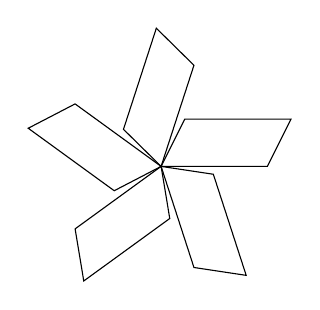
\begin{tikzpicture}[scale = 1.5]
            % Draw five petals rotated around the origin
            \foreach \angle in {0,72,...,288} {
            \begin{scope}[rotate=\angle]
                \petal
            \end{scope}
            }
        \end{tikzpicture}\\\hline
    \end{tabular}
\end{minipage}
	\begin{enumerate}
		\item Par quelle valeur doit-on compléter la ligne 2 du bloc \og Fleur \fg{} ci-dessus ? 
\emph{Aucune justification n'est attendue.}
		\item Expliquer le choix de la valeur \og 72 \fg{} dans la ligne 4.
		\item On modifie le bloc \og Fleur \fg{} pour construire le motif suivant:

\begin{center}
    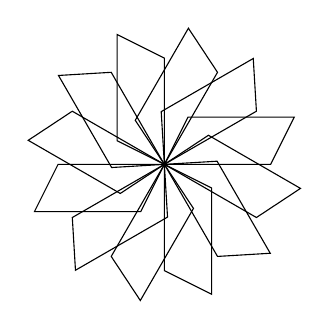
\begin{tikzpicture}[scale = 1.5]
        % Draw the parallelogram rotated around the origin 12 times at 30-degree intervals
        \foreach \angle in {0,30,...,330} {
            \begin{scope}[rotate=\angle]
                \petal
            \end{scope}
        }
    \end{tikzpicture}
\end{center}

Quelles sont alors les modifications à apporter aux lignes 2 et 4 du bloc \og Fleur\fg{} ? \emph{Aucune justification n'est attendue}.
	\end{enumerate}
\end{enumerate}